\begin{frame}
  \frametitle{MatLabb}
  \framesubtitle{Overgripande beskrivning}
  \begin{itemize}
  \item<1-> Graphical User Interface.
  \item<2-> Fyra olika vyer.
  \end{itemize}
\end{frame}

\begin{frame}
  \frametitle{MatLabb}
  \framesubtitle{Sökvyn}
  \begin{figure}[H]
    \centering 
    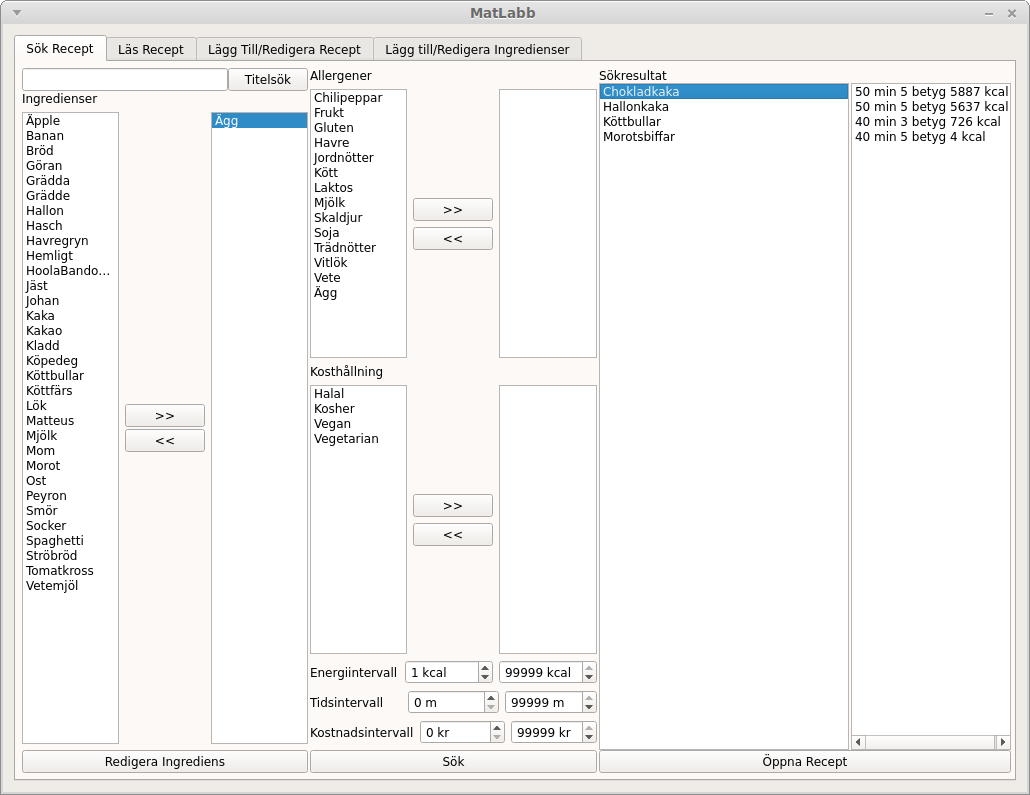
\includegraphics[scale=0.25]{sok_recept.png} 
    %\caption{Entity-Relationship diagram} 
  \end{figure}
\end{frame}

\begin{frame}
  \frametitle{MatLabb}
  \framesubtitle{Receptvyn}
  \begin{figure}[H]
    \centering 
    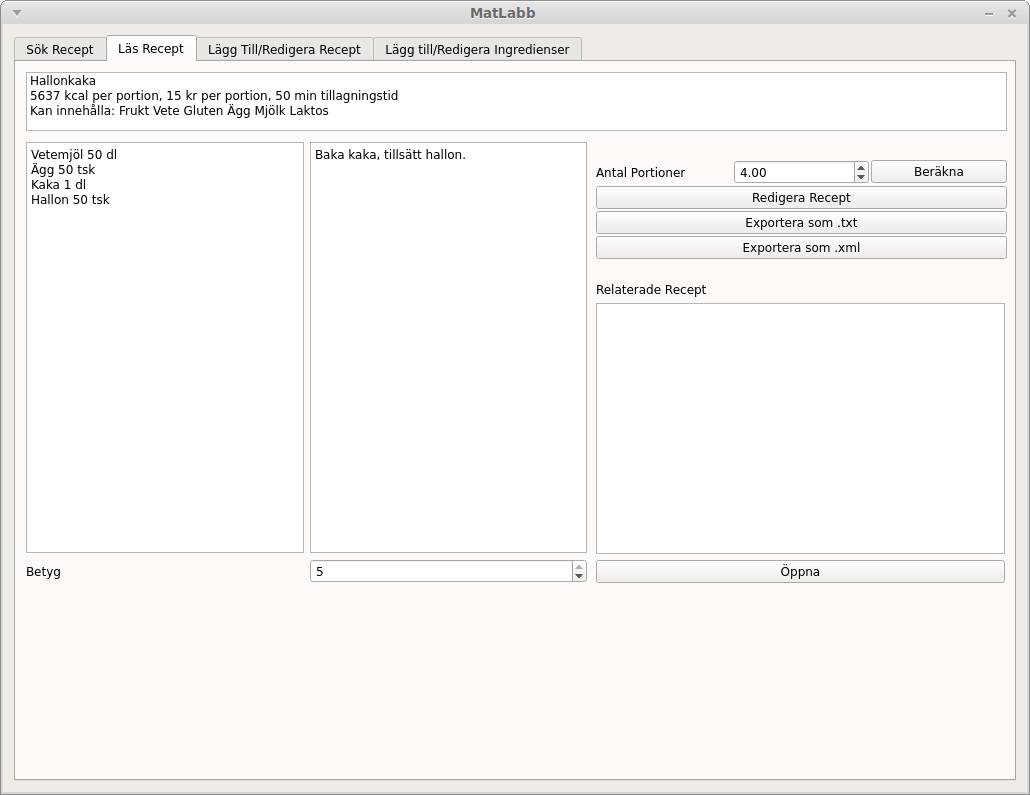
\includegraphics[scale=0.25]{las_recept.png} 
    %\caption{Entity-Relationship diagram} 
  \end{figure}
\end{frame}

\begin{frame}
  \frametitle{MatLabb}
  \framesubtitle{Receptredigeringsvyn}
  \begin{figure}[H]
    \centering 
    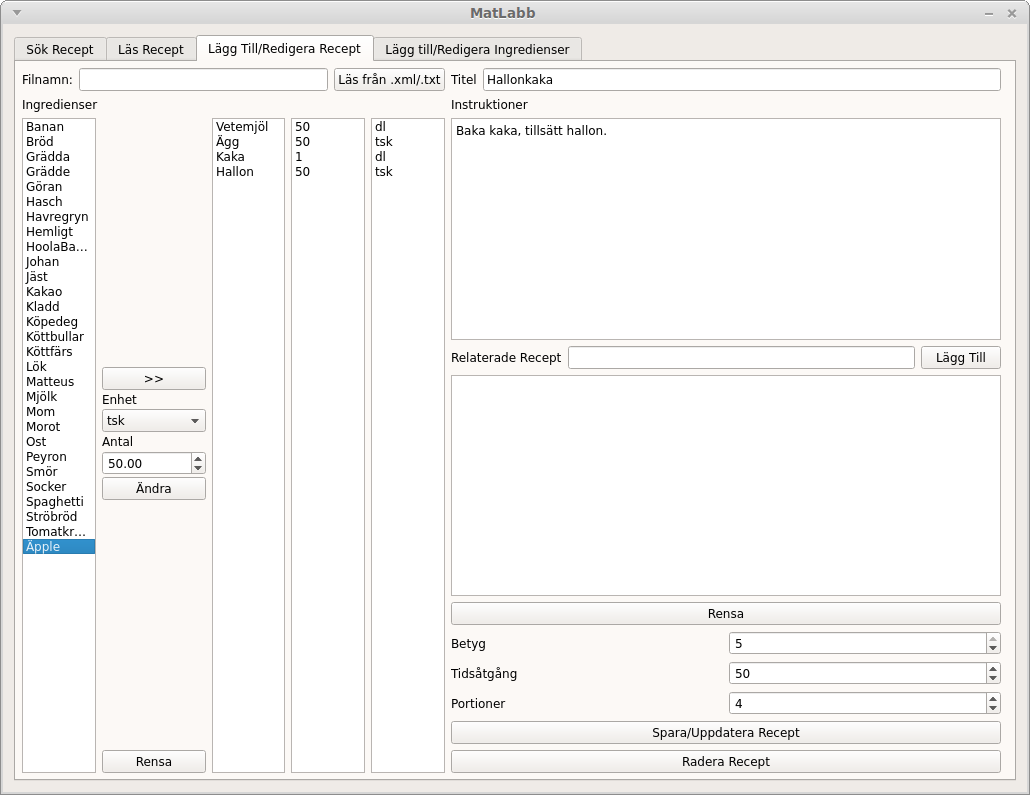
\includegraphics[scale=0.25]{lagg_till_recept.png} 
    %\caption{Entity-Relationship diagram} 
  \end{figure}
\end{frame}

\begin{frame}
  \frametitle{MatLabb}
  \framesubtitle{Ingrediensredigeringsvyn}
  \begin{figure}[H]
    \centering 
    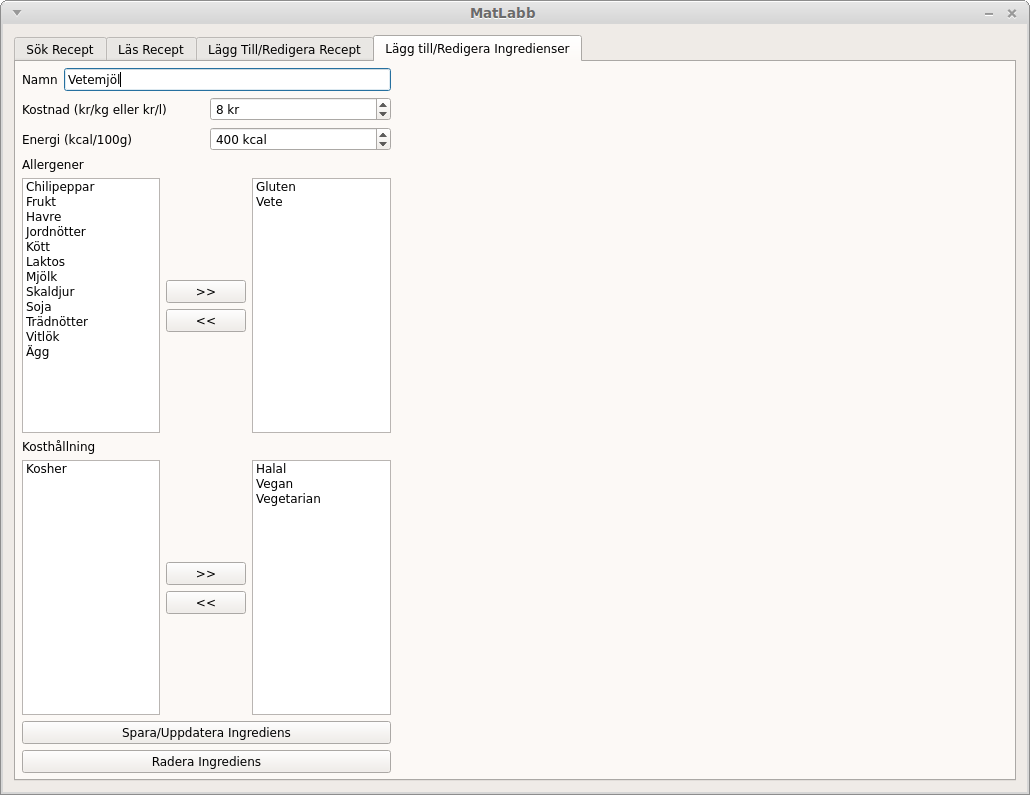
\includegraphics[scale=0.25]{lagg_till_ingrediens.png} 
    %\caption{Entity-Relationship diagram} 
  \end{figure}
\end{frame}
